\documentclass[WHATMANUAL.tex]{subfiles}

\begin{document}

\section{Downloading and formatting data from the CDCD}

\subsection{Introduction}

The Canadian Daily Climate Database (CDCD) contains daily data for air temperature and precipitation dating back to 1840 to the present for about 8450 stations distributed across Canada. Data can be downloaded manually on the Government of Canada website (\url{www.climate.weather.gc.ca}) for each year individually and saved in a csv file. This process involves a lot of repetitive manipulations and is a time consuming task. Moreover, the re-organization of the individual data files, saved for each year separately, in a more convenient format can also represent a tedious task when done manually. Alternately, it is possible to order a DVD containing the entire database for a small fee. This option has the disadvantage of only providing an image in time as data cannot be updated.  

WHAT alleviates this process by providing a graphical interface to the online CDCD that allows to query for stations interactively using location coordinates, download the available data for the selected weather stations, and automatically organize the data in a format compatible with WHAT. These features are available in the \emph{Download Data} tab shown in \cref{fig:tab_dwnldData}. This tab consists of a toolbar located at the top of the interface, an area where are displayed the current list of weather stations for which data can be downloaded, and a side-panel to the right where can be manage the formatting of the weather data files that were downloaded for each year individually. 

\subsection{Searching for weather stations}

Before any weather data can be downloaded from the online CDCD, a list of stations must first be provided to WHAT. This can be done by selecting an already existing list of stations (files with a ``lst'' extension) by clicking on the opened document~{
\includegraphics[height=2ex]{img/open_file}} icon located in the toolbar. 

Alternatively, it is possible to search for weather stations in the online CDCD by clicking on the magnifying glass~{
\includegraphics[height=2ex]{img/search}} icon in the toolbar. This will open a new dialog window (see \cref{fig:Screenshot_search4stations}) where it is possible to search for weather stations located within a given radius around a set of location coordinates (latitude and longitude) in decimal degrees. It is possible to further narrow down the search by including only stations with data available within a given period and/or with data available for a minimum number of years.

\begin{figure}[!hb]
    \setlength{\fboxsep}{0pt}
    \ffigbox[\FBwidth]
    {
     \caption{Screenshot of WHAT v4.1.7-beta in Ubuntu-Linux 15.04 showing the \emph{Download Data} tab.}
     \label{fig:tab_dwnldData}
    }
    {
     \fbox{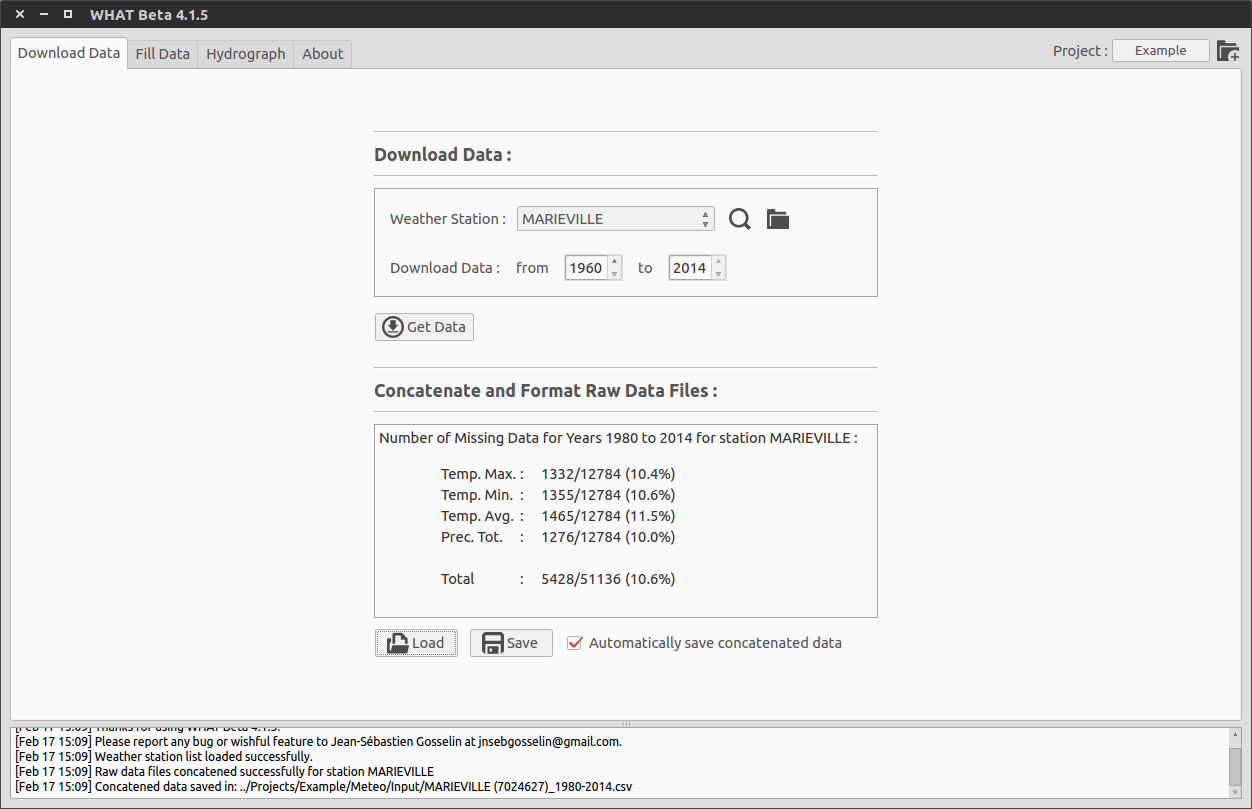
\includegraphics[width=0.75\textwidth]{img/WHAT_Screenshot000}}
    }
    
    \vspace{2em}
    
    \ffigbox[\FBwidth]
    {
     \caption{Screenshot of WHAT v4.1.7-beta in Ubuntu-Linux 15.04 showing the \emph{graphical interface} to the online CDCD database.}
     \label{fig:Screenshot_search4stations}
    }
    {
     \fbox{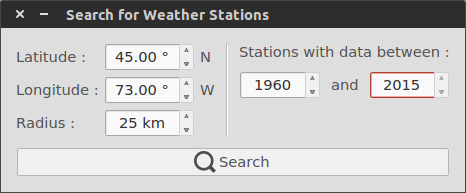
\includegraphics[width=0.75\textwidth]{img/WHAT_Screenshot_search4stations}}
    }
\end{figure}

When all the parameters have been specified, the search for weather stations in the online CDCD can be initiated by clicking on the \emph{Search Stations}~{
\includegraphics[height=2ex]{img/search}} button. The resulting stations are automatically displayed in a table, along with information regarding their proximity to the location coordinates used for the search, the years for which data are available, their province, and their climate ID. Selecting stations and clicking on the \emph{Add Stations}~{
\includegraphics[height=2ex]{img/add2list}} button will add them to the current list of weather stations displayed in the \emph{Download Data} tab.

It is possible to remove any weather station from the current list by selecting them and clicking on the toolbar eraser~{
\includegraphics[height=2ex]{img/erase}} icon. The station list can be saved by clicking on the toolbar floppy disk~{
\includegraphics[height=2ex]{img/save}} icon. Alternatively, it is also possible to generate a list of weather stations by creating manually a lst file without using the graphical interface. This is done by retrieving station information from their unique url directly on the government of Canada website (\url{www.climate.weather.gc.ca}) and saving the information in a tsv (tabular-separated values) text file with a ``lst'' extension. A detailed example is presented in \cref{app:custom_station_list}

\subsection{Downloading the weather data}

Daily weather data can be downloaded from the online CDCD by selecting the desired stations from the list displayed in the \emph{Download Data} tab and clicking on the toolbar icon with the encircled downward arrow~{
\includegraphics[height=2ex]{img/download}}. Data will be downloaded for the years specified for each selected station and the results will be  saved automatically as a csv (comma-separated values) file in the \emph{Raw} folder (see section~\ref{subsec:folder_structure}). Weather data for a given station won't be downloaded for the years for which a data file already exist in the \emph{Raw} folder. Detailed information about the downloading process are printed in the console area located at the bottom of the interface (see section~\ref{sec:GUI_overview}). The downloading process can be stopped at any time by clicking on the stop~{
\includegraphics[height=2ex]{img/process-stop_alternate}} icon that appears in the toolbar as soon a downloading task is started.

\subsection{Formatting the weather data}\label{subsec:formatting_weather_data}

WHAT automatically formats the data as soon as they have been successfully downloaded for a given weather station. To do this, data from each annual file are put together end to end in chronological order. Only the data related to air temperature (mean, max and min) and total precipitation are kept. In addition, days with missing data in the dataset are filled with a NaN (not a number) value. Finally, information on the number of days with missing data for each meteorological variable are displayed in the right side-panel. Alternatively, it is possible to open and format previously downloaded weather data files by clicking on the \emph{Load}~{
\includegraphics[height=2ex]{img/open_file}} button in the right side-panel and selecting the desired files from the dialog window that will open.

By default, WHAT will automatically save the formatted data in a single tsv (tabular-separated values) file in the \emph{Input} folder (see section~\ref{subsec:folder_structure}). The automatic saving of the formatted data series can be disabled by unchecking the \emph{Automatically save concatenated data} option. From the right side-panel, it is then possible to navigate through the datasets that were formatted over the course of a given session using the left-right arrows and save any dataset manually by clicking on the save~{
\includegraphics[height=2ex]{img/save}} button.

\section{Filling the gaps in daily weather records}\label{guide-gapfilling}

\subsection{Introduction}

Climate data are useful in several fields of Earth sciences, including hydrology, hydrogeology and agronomy. However, climate datasets are, most of the time, incomplete. This can represent a major hindrance in various applications, such as for hydrological or hydrogeological model simulations that heavily depend on these data.

Filling the gaps in weather datasets can quickly become a tedious task as the size of the data records and the number of stations increase. Moreover, it can also be rather complex when aspects such as time-efficiency of the method, accuracy of the estimated missing values, and preservation of the statistical properties of the weather time series (probability distribution and normals) are taken into account. This is particularly true for the estimation of missing daily precipitation data because of their high spatial and temporal variability \citep{simolo_improving_2010}.

WHAT addresses this issue by providing an automated, robust, and efficient method to quickly and easily fill the gaps in the daily weather datasets from the files that were produced as described in \cref{subsec:formatting_weather_data}. It is also possible to fill the gaps in weather datasets from files that were not produced with WHAT, provided that the data are formatted in the right format (see \cref{sec:weather_datafile_format}). In addition, WHAT includes the framework to easily validate and assess the uncertainty of the estimated missing values with a cross-validation resampling technique. These features are available in the \emph{Fill Data} tab shown in \cref{fig:tab_fillData}. This tab consists in a side-panel to the left where the gapfilling procedure can be managed and configured and an area to the right where various outputs are displayed.

\subsection{Loading the weather data files}\label{subsec:creating_list}

When starting WHAT or when a project is opened, the content of the \emph{Input} folder is automatically scanned for weather data files. The results are displayed in a list of weather stations, located under the label \emph{Fill data for weather station}. A summary of the number of days with missing data for each dataset is also produced and displayed in the tab \emph{Missing Data Overview} of the display area, to the right. The icon with the circular arrows~{
\includegraphics[height=2ex]{img/refresh2}}, located next to the list of stations, can be clicked to re-scan the \emph{Input} folder for new weather data files to update the list of stations and the summary. 

\begin{figure}[!ht]
    \setlength{\fboxsep}{0pt}
    \ffigbox[\FBwidth]
    {
     \caption{Screenshot of WHAT v4.1.7-beta in Ubuntu-Linux 15.04 showing the \emph{Fill Data} tab.}
     \label{fig:tab_fillData}
    }
    {
     \fbox{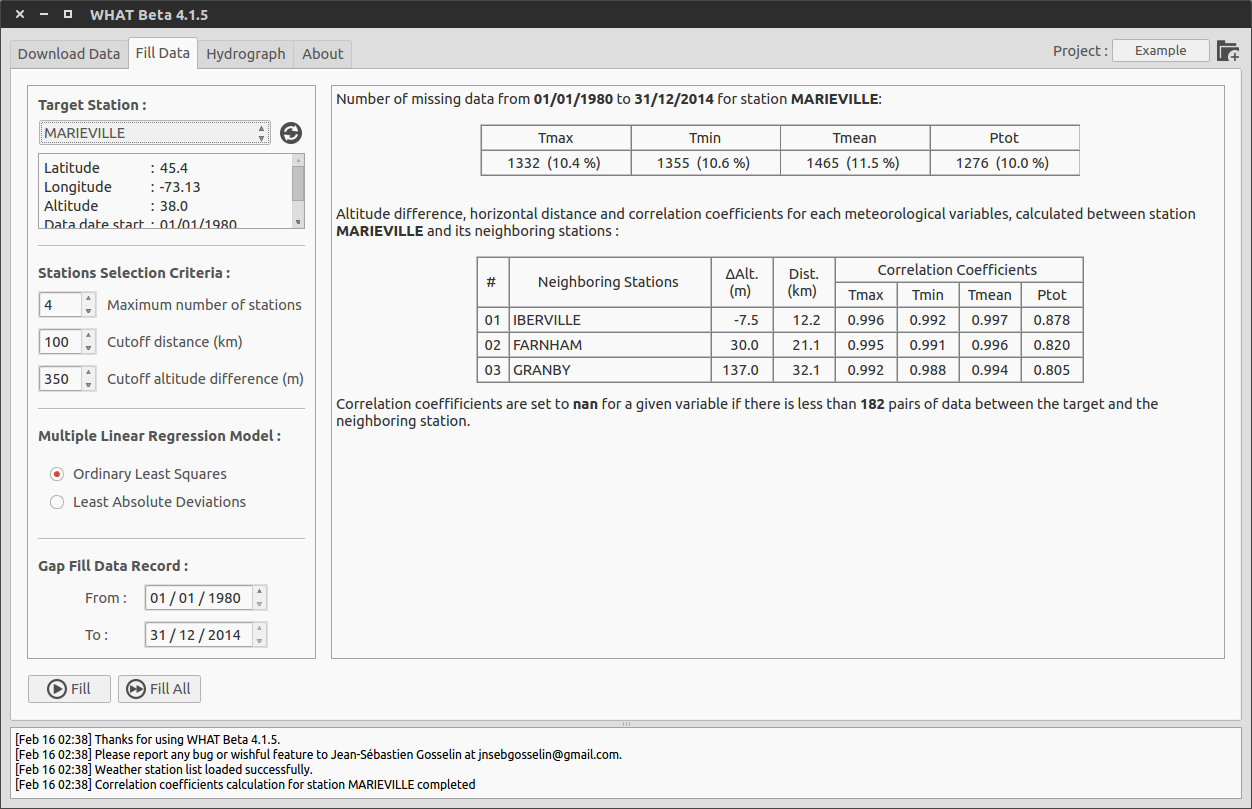
\includegraphics[width=0.75\textwidth]{img/WHAT_Screenshot001}}
    }
\end{figure}

\subsection{Setting the model parameters}

The first step is to select the station for which missing values in the dataset need to be filled. This is done from the drop-down list located under the \emph{Fill data for station} section shown in \cref{fig:fill_data_for}. Under this list are automatically posted information about the currently selected weather station. It is also possible to define the period for which the data of the selected station will be filled by editing the dates fields located next to the \emph{From} and \emph{To} labels. By default, dates are set as the first and the last date for which data are available for any of the stations of the list.

The method used to estimate the missing data for the selected weather station consists in the generation of a multiple linear regression (MLR) model, using synchronous data from selected neighboring stations from the list. The neighboring stations are selected mainly on the basis of the correlation coefficients computed between their data and those of the selected weather station. The values of these coefficients are automatically displayed in the table located in the right side of the interface when a new weather station is selected from the list. Moreover, among the selected neighboring stations, the ones with the highest correlation coefficients have more weight in the model than those with weak correlation coefficients. For this reason, correlation coefficients that fall below a value of 0.7 are shown in red in the table, as a guidance for the user. There are several settings that can be used to control the selection of the neighboring stations, the generation of the MLR model, and the outputs of the gapfilling procedure. An overview of these settings is presented below.

\begin{figure}[!h]
    \setlength{\fboxsep}{0pt}
    \thisfloatsetup{capbesideposition={right,bottom},
                    objectset=raggedright}
    \floatbox[\capbeside]{figure}[\FBwidth]
	{
	 \caption{Screenshot of WHAT v4.1.7-beta in Ubuntu-Linux 15.04 showing the \emph{Fill data for station} section. For this setup, missing values in the datasets of the selected weather station (MARIEVILLE) would be filled for the 01/01/1980 to 31/12/2015 period.}
	 \label{fig:fill_data_for}
	}
	{
	 \fbox{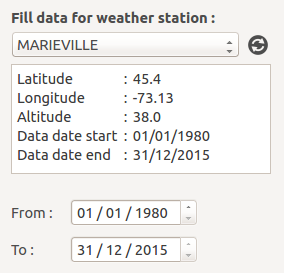
\includegraphics[width=0.35\textwidth]{img/WHAT_Screenshot_Fill_data_for.png}}
	}
\end{figure}

\paragraph{Station Selection Criteria :} A MLR model is generated for each day for which a data is missing in the dataset of the selected station. This is done because the number of neighboring stations with available data can vary in time. Therefore, for a given date with missing data in the dataset of the selected station, the neighboring stations are selected in decreasing order of their correlation coefficients. Neighboring stations that also have a missing data at this particular date are excluded from the selection process. The maximum number of station that are selected for the generation of the MLR model can be specified in the \emph{Nbr. of stations} field, located in the \emph{Stations Selection Criteria} menu shown in \cref{fig:selection_criteria}. The number of neighboring station that is selected by default is 4. If for a given date, all the neighboring stations have missing data synchronously with the selected station, a NaN value is kept in the dataset at this particular date. 

Moreover, the correlation between the data of two stations will, in general, decreases as the distance and the altitude difference between them increase. Therefore, the fields \emph{Max. Distance} and \emph{Max. Elevation Diff.} allow to specify thresholds for the distance and altitude difference. Neighboring stations exceeding either one of these thresholds will not be used to fill the gaps in the dataset of the selected station. The default values for the distance and altitude difference are set to \SI{100}{km} and \SI{350}{m}, respectively, based on a literature review \citep{tronci_comparison_1986,xia_forest_1999,simolo_improving_2010}. The horizontal distances and elevation differences calculated between the selected station and its neighbors are shown in the table to the right, alongside the correlation coefficients. The values that exceed their corresponding threshold are shown in red.

\begin{figure}[!hb]
    \setlength{\fboxsep}{0pt}
    \thisfloatsetup{capbesideposition={right,bottom},
                    objectset=raggedright}
    \floatbox[\capbeside]{figure}[\FBwidth]
	{
	 \caption{Screenshot of WHAT v4.1.7-beta in Ubuntu-Linux 15.04 showing the \emph{Advanced Settings} menu.}
	 \label{fig:selection_criteria}
	}
	{
	 \fbox{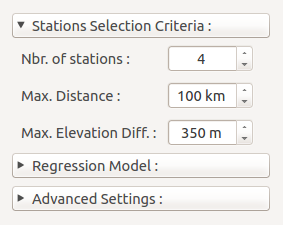
\includegraphics[width=0.35\textwidth]{img/WHAT_Screenshot_selection_criteria}}
	}
\end{figure}

\paragraph{Regression Model :} It is possible to select whether the MLR model is generated using a Ordinary Least Squares (OLS) or a Least Absolute Deviations (LAD) criteria from the \emph{Regression Model} menu shown in \cref{fig:regression_model}. A regression based on a LAD is more robust to outliers than a regression based on a OLS, but is more expensive in computation time.

\begin{figure}[!ht]
    \setlength{\fboxsep}{0pt}
    \thisfloatsetup{capbesideposition={right,bottom},
                    objectset=raggedright}
    \floatbox[\capbeside]{figure}[\FBwidth]
	{
	 \caption{Screenshot of WHAT v4.1.7-beta in Ubuntu-Linux 15.04 showing the \emph{Regression Model} menu.}
	 \label{fig:regression_model}
	}
	{
	 \fbox{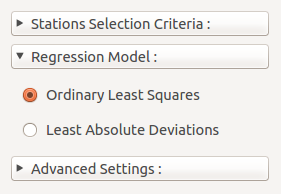
\includegraphics[width=0.35\textwidth]{img/WHAT_Screenshot_regression_model}}
	}
\end{figure}

\paragraph{Advanced Settings :} It is possible to automatically estimate and add the daily Potential Evapotranspiration (ETP) to the output data file produced at the end of the gapfilling procedure of the selected station. This option is enabled by checking the \emph{Add ETP to data file} option in the menu \emph{Advanced Settings} shown in \cref{fig:adv_settings}. The daily ETP is estimated with a method adapted from \cite{thornthwaite_approach_1948}, using the daily mean air temperature time series of the selected station. Alternatively, it is possible to add manually the ETP to an existing weather data file by clicking on the open file~{
\includegraphics[height=2ex]{img/open_file}} icon located next to the \emph{Add ETP to data file} option.

The \emph{Full Error Analysis} option can be checked to perform a cross-validation resampling analysis during the gapfilling procedure. The results from this analysis can be used afterward to estimate the accuracy of the method. This option is discussed in more details in \cref{subsec:uncertainty}.

\begin{figure}[!ht]
    \setlength{\fboxsep}{0pt}
    \thisfloatsetup{capbesideposition={right,bottom},
                    objectset=raggedright}
    \floatbox[\capbeside]{figure}[\FBwidth]
	{
	 \caption{Screenshot of WHAT v4.1.7-beta in Ubuntu-Linux 15.04 showing the \emph{Advanced Settings} menu.}
	 \label{fig:adv_settings}
	}
	{
	 \fbox{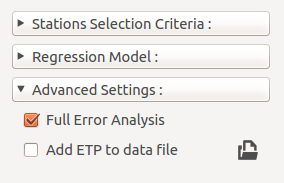
\includegraphics[width=0.35\textwidth]{img/WHAT_Screenshot_advanced_settings}}
	}
\end{figure}

\subsection{Filling the gaps in the data}\label{subsec:filling_the_gaps}

The automated procedure to fill the gaps in the dataset of the selected weather station can be started by clicking the button \emph{Fill}~{
\includegraphics[height=2ex]{img/fill_data}} located at the bottom of the left side-panel. It is also possible to run this procedure in batch mode to fill the gaps in the datasets of the entire list of weather station by clicking on the button \emph{Fill All Stations}~{
\includegraphics[height=2ex]{img/fill_all_data}}. The parameters for the gap filling procedure will, however, be the same for all the stations.

Once the process is completed for a station, the resulting gapless daily weather dataset is automatically saved in a tsv (tabular-separated values) file with the extension ‘‘.out’’ in the \emph{Output} folder (see \cref{subsec:folder_structure}). The file is named after the weather station name, climate ID, and first and last year of the dataset. For example, the resulting output file for the station MARIEVILLE in \cref{fig:tab_fillData} would be ‘‘MARIEVILLE (7024627) 1980-2015.out’’.  In addition, detailed information on the values estimated for filling the gaps in the data are saved in a file with the same name as the ‘‘.out'' file, but with a ‘‘.log'' extension. Information includes, the names of the neighboring stations, the values of the data used for the estimations, as well as the expected uncertainty of the estimates.

\subsection{Uncertainty of the estimated values}\label{subsec:uncertainty}

By default, each time a new MLR model is generated to estimate a missing value in the dataset of the selected station, the model is also used to predict the values in the dataset that are not missing. The accuracy of the MLR model is then approximated by computing a Root-Mean-Square Error (RMSE) between the values estimated with the model and the respective non-missing observations in the dataset of the selected station. The RMSE thus calculated is saved, along with the estimated value, in the ``.log'' file.

When the \emph{Full Error Analysis} option in the \emph{Advanced Settings} menu is enabled, WHAT will also perform a cross-validation resampling procedure to estimate the accuracy of the model, in addition to fill the gaps in the dataset. More specifically, the procedure consists in estimating alternately a weather data value for each day of the selected station's dataset, even for days for which data are not missing. Before estimating a value for a given day, the corresponding measured data in the dataset of the selected station is temporarily discarded to avoid self-influence of this observation on the generation of the MLR model. The model is then generated and used to estimate a value on this given day and the corresponding observed data is put back in the dataset of the selected station. When a value for every day of the dataset has thus been estimated, the estimated values are saved in a tsv (tabular-separated values) file in the \emph{Output} folder with the extension ‘‘.err’’, along with the ‘‘.log’’ and ‘‘.out’’ files described in \cref{subsec:filling_the_gaps}. The accuracy of the method can then be estimated by computing the RMSE between the estimated weather data and the respective non-missing observations in the original dataset of the selected station. Activating this feature will significantly increase the computation time of the gap filling procedure, especially if the least absolute deviation regression model is selected, but can provide interesting insights on the performance of the procedure for the specific datasets used for a project.

\end{document}

%It is possible, from the \emph{Fill Data} tab (see \cref{fig:tab_fillData}), to automatically fill the gaps in the daily weather datasets from the files that were produced as described in \cref{subsec:formatting_weather_data}. It is also possible to fill the gaps in weather datasets from files that were not produced with WHAT. The data must, however, be formatted in the right format and saved as a tsv file in the \emph{Input} folder. A detailed description of the weather data file format used in WHAT is presented in \cref{sec:weather_datafile_format}.

%It has been demonstrated that the MLR method outperforms most of the commonly used techniques for the estimation of missing data in daily meteorological records \citep{eischeid_quality_1995,eischeid_creating_2000,xia_forest_1999}. 